\documentclass{article}
\usepackage{graphicx}
\usepackage{authblk}
\usepackage{amsmath}


\begin{document}
\title{THEORETICAL NEUROSCIENCE \\ EXERCISE 3}
\date{\today}
\author[1]{\c{S}eyma Bayrak\thanks{seyma.bayrak@st.ovgu.de}}
\affil[1]{\footnotesize  Otto von Guericke University of Magdeburg}
\maketitle


\section*{Part 1}
The purpose of this exercise is to provide an imaginary step-functioned current, $i_{e}$, to the neuron, and then to analyze the behavior of membrane voltage, $V_{m}$.The whole electrical activity of neuron is thought to be a parallel connected circuit with resistor and capacitor elements. This assumption leads us to use ``Single Compartment Model -SCM'', which basically models $V_{m}$, with the already known value of input current and time range. The input current is modelled as given by equation 1.

\begin{equation}
 i_{e}=0,\,\,\,\,\,  0\le t <\dfrac{T}{4} \,\,\,and\,\,\, i_{e}=i_{0},\,\,\,\, \frac{3T}{4}<t\le T
\end{equation}

The step functioned current amplitude is $i_{e}$ is given as 12 $nA/mm^{2}$, the current per unit membrane area, the total time range is between 0 and 500 $ms$. Subsequent to the modeling of input current and time vectors, the Euler’s simple integration method is programmed to find out membrane potential. A brief mathematical introduction of Euler’s Method is provided as the following,

\begin{equation}
 \dfrac{dV_{m}}{dt}=\dfrac{1}{\tau_{m}}[V_{\infty}(t)-V_{m}(t)] \,\, \longrightarrow \,\, dV_{m}=\dfrac{1}{\tau_{m}}[V_{\infty}(t)-V_{m}(t)].dt
\end{equation}

\begin{equation}
V_{m}(t+dt)=V_{m}(t)+dV_{m}
\end{equation}

where $\tau_{m}$ denotes so called ``time constant'', equivalent to the multiplication of resistivity and capacitance, both per unit membrane area, $\tau_{m}=r_{m}.c_{m}$. The equilibrium potential $V_{\infty}$ is defined in this exercise as the reversal potential $E_{L}$ added to classical Ohm`s Law potential, $V_{\infty}=r_{m}i_{e}(t)$. 

\begin{equation*}
r_{m}=1.5 M \Omega mm^{2}\,\,\,\,\,c_{m}=20nF/mm^{2}\,\,\,\,\,E_{L}=-65mV
\end{equation*}

\begin{center}
 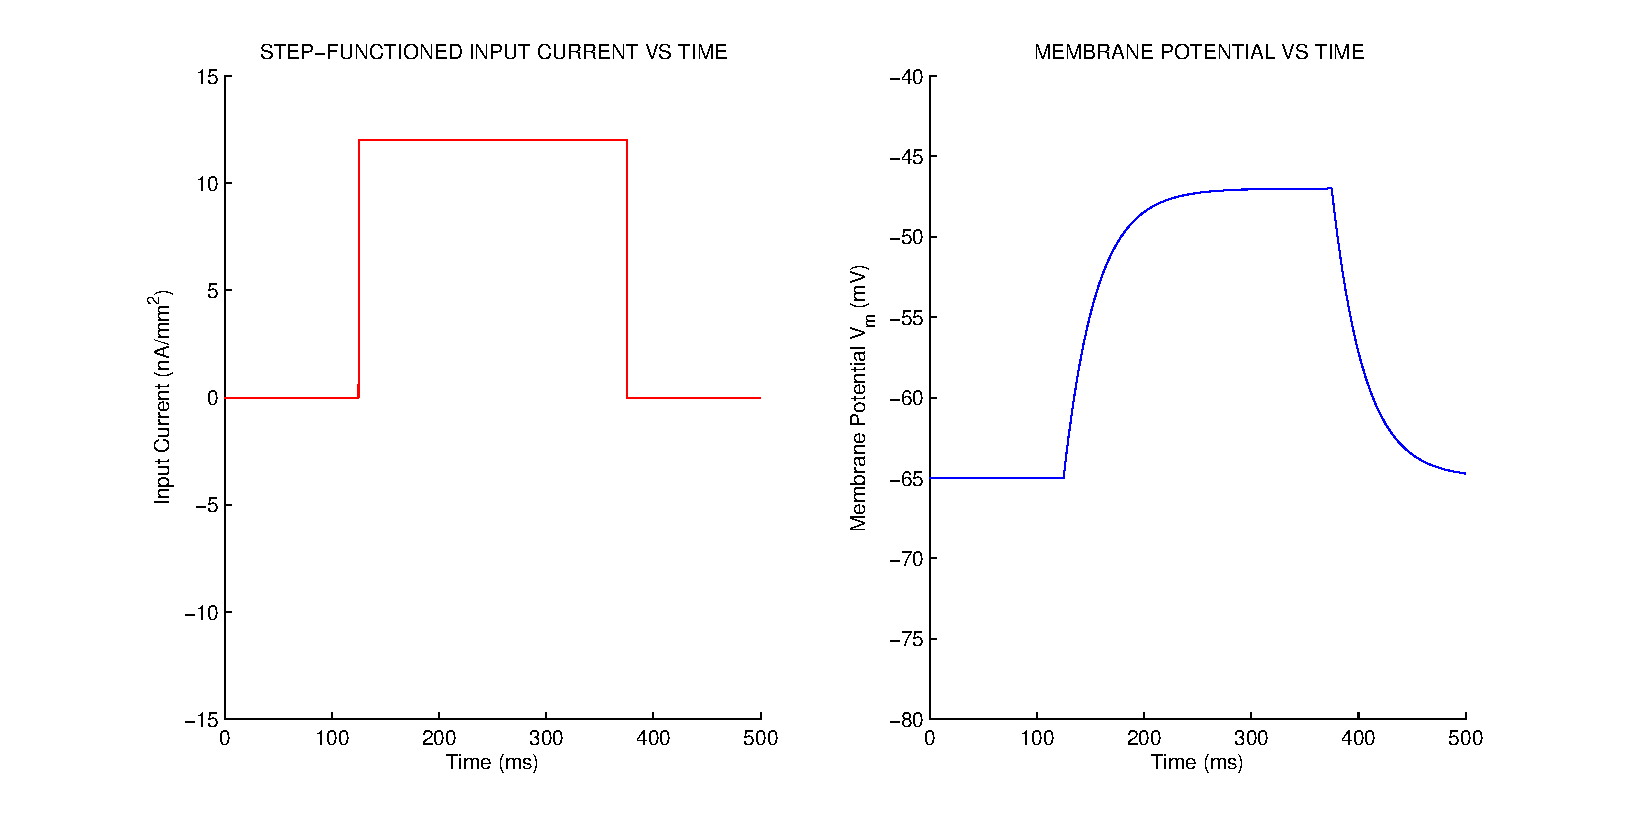
\includegraphics[width=\textwidth]{q7.eps}
 % q7.eps: 0x0 pixel, 300dpi, 0.00x0.00 cm, bb=  -86   231   682   610
Graph 1, The analysis of membrane potential caused by a step functioned input current, $V_{m}$ reaches to the maximum value of -47 mV, which is equals to the $V_{\infty}$ as expected.
\end{center}


\section*{Part 2}
The second part of exercise is much more interesting, now the imaginary action potentials are also taken into account, and we are even more close to the reality. Whenever the $V_{m}$ value equals to or exceeds the thereshold potential $V_{th}$, it suddenly falls down to level of reset potential $V_{reset}$. Therefore, $V_{m}$ is expected to have some ``spikes'' at the times on which the action potential occurs. The values for $V_{th}$ and $V_{reset}$ are given below. The new behavior of membrane potential with spikes can seen on Graph 2.

\begin{equation*}
V_{th}=-50 mV \,\,\,\,\,\,\,\,\,\,V_{reset}=-65 mV
\end{equation*}

The spikes occur subsequently at the times at 178.5 ms, 232.2 ms, 285.9 ms, and lastly 339.6 ms.The time interval between spikes $t_{isi}$ are all the same and it equals to 53.7 ms.The spike rate $r_{isi}$ is 0.0186 $ms^{-1}$, it is calculated by the formula of $r_{isi}=1/t_{isi}$.

\section*{Part 3}

The last part of exercise asks for calculating the time interval and time rate between spikes for the varying input currents. The amplitude of input current is changed continuosly from 24 $nA/mm^{2}$ to 0 and the values of $t_{isi}$ and $r_{isi}$ are recorded as shown in the table 1. 

\begin{center}
 
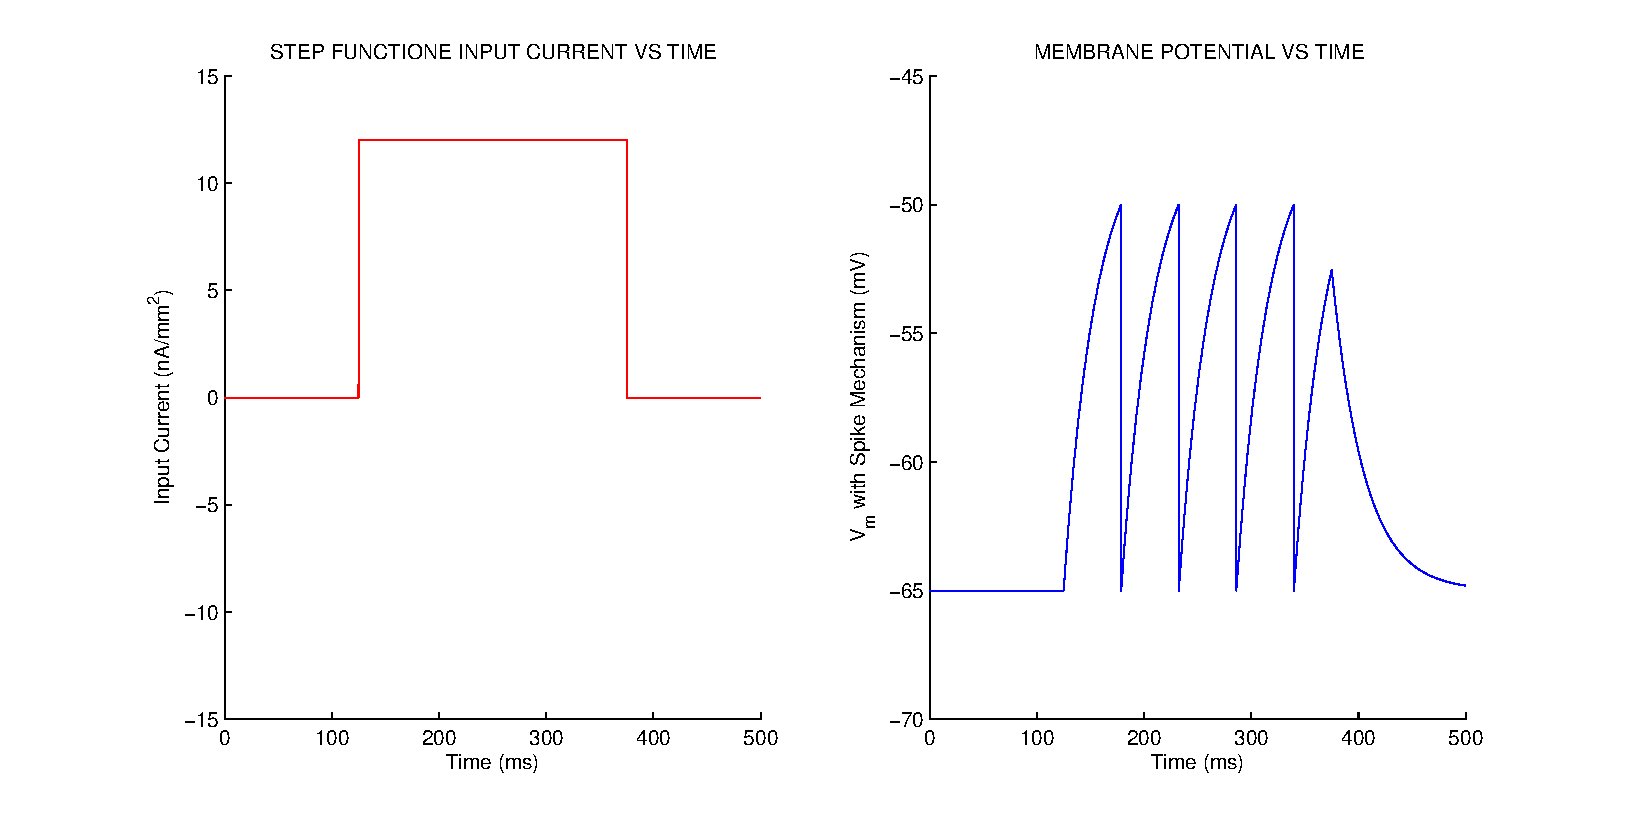
\includegraphics[width=\textwidth]{q8.eps}
 % q7.eps: 0x0 pixel, 300dpi, 0.00x0.00 cm, bb=  -86   231   682   610

Graph 2, The new $V_{m}$ with spikes, when it reaches to -50 mV,  drops to -65 mV. After the discontinuity, it turns to be a lower value.
\end{center}

\begin {table} [h]
\caption { The effect of varying input current amplitute on spike intervals and spike rates} \label{tab:title}
\begin{center}
  \begin{tabular}{ l | c | r }


    \hline
$i_{0}$ & $t_{isi}$ & $r_{isi}$\\ \hline \hline
 
    24 & 16.2 & 0.0617 \\ \hline
    22 & 18.2 & 0.0549 \\ \hline
    20 & 20.8 & 0.0481 \\ \hline
    18 & 24.3 & 0.0412 \\ \hline
    16 & 29.4 & 0.0340 \\ \hline
    14 & 37.6 & 0.0266 \\ \hline
    12 & 53.7 & 0.0186 \\ \hline
    10 & 71.9 & 0.0139 \\ \hline
  10.5 & 91.2 & 0.0110 \\ \hline



  \end{tabular}
\end{center}

\end{table}

\section*{Discussion}

The purpose of this exercise is to understand the ``The Leaky Integrate and Fire Model - LIF'' for the neurons, which is basically the analysis of membrane potential with imaginary action potentials of neuron. Without any action potential, $V_{m}$ increases continuosly exponential up to the equilibrium potential $V_{\infty}=-47 mV$ as the input current has a value rather than zero, and then decreases exponentailly to its initial value, $-65 mV$, as seen in Graph 1. 

However, when the action potentials are considered to occur, $V_{m}$ changes to be increased exponentially, only as long as it is lower than the threshold potential $V_{th}$. At the point at which $V_{m}$ exceeds or eqauls to $V_{th}=-50 mV$, it suddenly drops to its original value of $-65 mV$ . This behavior repeats itself several times until the input current is again 0. Graph 2 indicates spikes created by LIF model. It also shows that, after discontinuity, the last peak  of $V_{m}$ fells down continuosly back to its initial value; but this time it starts already decreasing before being reached to $V_{th}$.

The most important result of the exercise was to observe facts that, the lower the input current is to more time needed to create a new spike. $t_{isi}$ gets larger and $r_{isi}$ gets smaller, inversely to $t_{isi}$. Moreover, below a certain value of input current, there happens no spike mechanism at $V_{m}$ potential behavior. This specific point of $i_{0}$ is defined as ``input threshold'', and calculated as below. 

\begin{equation}
I_{e} \geq  \dfrac{V_{th}-E_{L}}{r}
\end{equation}

This value corresponds quantitively $10 nA/mm^{2}$ in this exercise, table 1 shows the last value of input current as $10.5 nA/mm^{2}$ applied to the neuron. Graph 3 is an exmaple of input current of $6 nA/mm^{2}$, as expected $V_{m}$ behaves as in SCM. 

\begin{center}

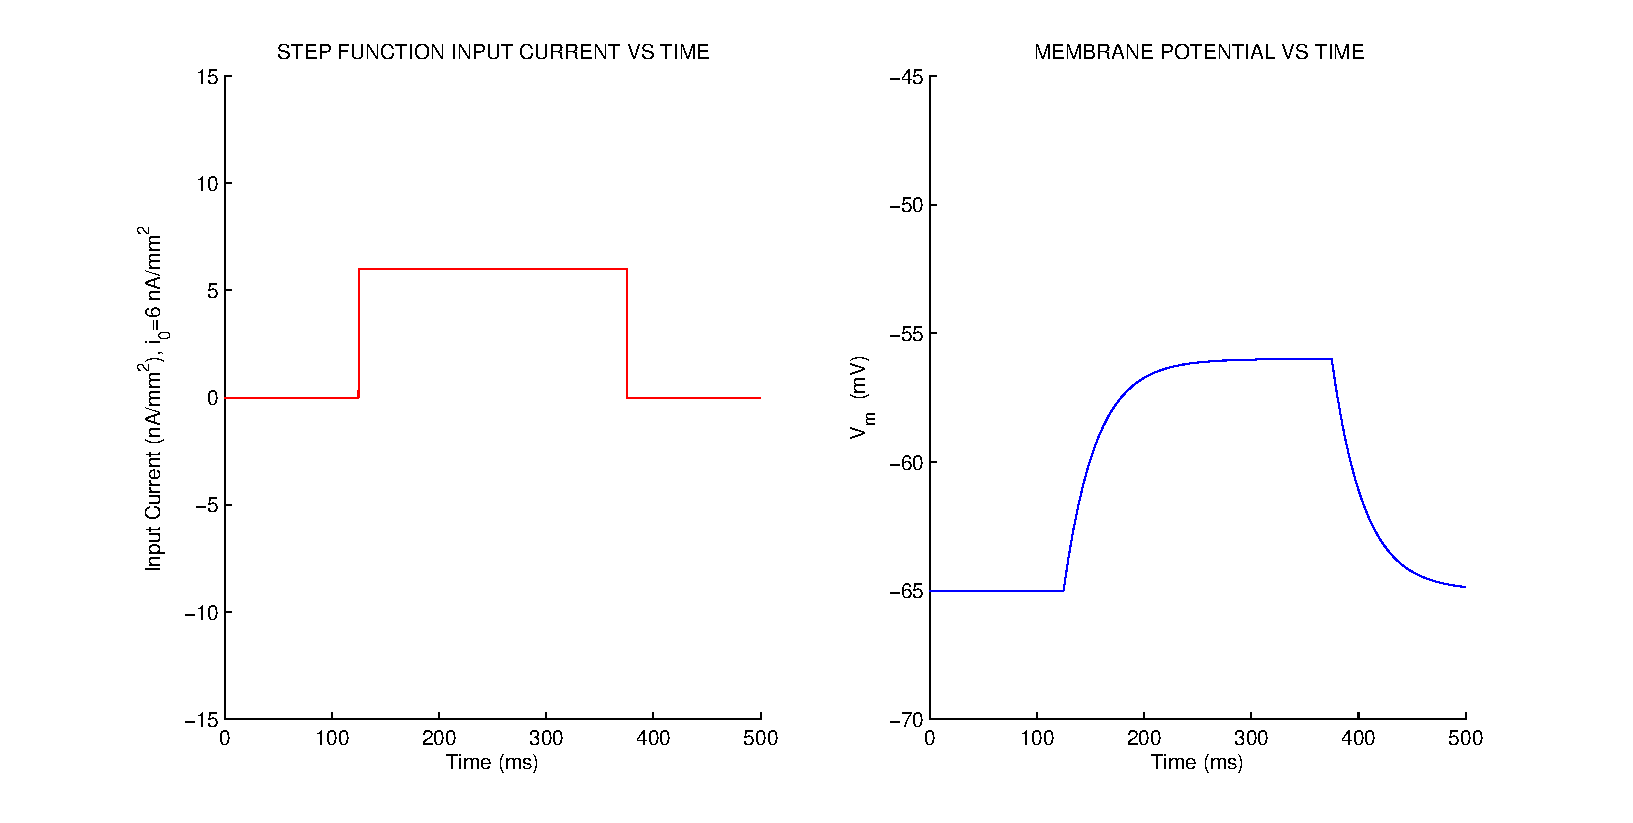
\includegraphics[width=\textwidth]{q10.eps}
 % q7.eps: 0x0 pixel, 300dpi, 0.00x0.00 cm, bb=  -86   231   682   610

Graph 3, Input current lower than $10 nA/mm^{2}$ yields $V_{m}$ to act as in SCM model.
\end{center}
Additional trials shows that the increment in $E_{L}$, or decrement in $c_{m}$, $\tau_{m}$ results in more frequent spikes.

\end{document}






